% Supplementary material for "When are triangles invisible?" — lives in the
% code repository (github.com/appleweiping/topo-flow-limits); referenced from
% the main paper. Compile: pdflatex supplement && pdflatex supplement.
\documentclass[11pt]{article}
\usepackage[margin=1.1in]{geometry}
\usepackage{amsmath,amssymb,amsthm}
\usepackage{graphicx}
\usepackage{bm}
\usepackage[hidelinks]{hyperref}
\graphicspath{{figures/}{../results/figures/}}

\renewcommand{\thesection}{S\arabic{section}}
\newtheorem{theorem}{Theorem}[section]
\newtheorem{proposition}[theorem]{Proposition}
\newtheorem{lemma}[theorem]{Lemma}
\newtheorem{corollary}[theorem]{Corollary}
\newtheorem{remark}[theorem]{Remark}

\DeclareMathOperator{\rank}{rank}
\newcommand{\B}{\bm{B}}
\newcommand{\R}{\mathbb{R}}
\newcommand{\E}{\mathbb{E}}
\newcommand{\Scal}{\mathcal{S}}
\newcommand{\Tcal}{\mathcal{T}}
\newcommand{\KL}{\mathrm{KL}}

\title{Supplementary Material for\\
``When Are Triangles Invisible? Fundamental Limits of\\
Higher-Order Structure Identifiability from Edge Flows''}
\author{Weiping Yan\\ \small University of Minnesota, Twin Cities}
\date{}

\begin{document}
\maketitle

\noindent
This supplement extends the main paper in three directions: \textbf{S1}
Fano-type converses for \emph{joint} support recovery (including a
signal-distribution-agnostic bound and a sub-Gaussian achievability
counterpart); \textbf{S2} identifiability under \emph{partial edge
observation}; \textbf{S3} \emph{plug-in} estimation of the variance parameters
and a fully adaptive detector. All statements are validated numerically by the
released test-suite; Section~\ref{sec:repro} maps every figure to its script.
Notation follows the main paper: $N$ snapshots, candidate set $\Tcal$ with
$p=|\Tcal|$, latent support $\Scal$ with $|\Scal|=k$, curl-SNR
$\rho=3\sigma_c^2/\sigma_n^2$, per-coordinate null/alternative variances
$v_0=3\sigma_n^2$, $v_1=v_0(1+\rho)$. Throughout S1--S2 the candidates are
pairwise edge-disjoint, so the curl coordinates are independent given
$\Scal$ and the triangle Gram matrix is $\bm G=3\bm I$.

\section{Fano-type converses for joint support recovery}\label{sec:fano}

The main paper's Theorem~1 is a \emph{single-triangle} converse: it bounds the
error of deciding one triangle's activity and yields the floor
$\rho^\star(N)=\Theta(\sqrt{\log(1/\delta)/N})$. Recovering the whole support
$\Scal$ among $\binom pk$ possibilities is harder. The next two theorems
quantify by how much.

We first record a reduction used by both proofs.

\begin{lemma}[Sufficiency of the curl coordinates]\label{lem:reduction}
Consider the model of the main paper (Eq.~(2)) with isotropic Gaussian noise
$\bm n_t\sim\mathcal N(0,\sigma_n^2\bm I)$, mutually independent
$(\bm a_t,\bm y_t,\bm h_t,\bm n_t)$, and \emph{arbitrary} laws for
$(\bm a_t,\bm y_t,\bm h_t)$ (Gaussianity is needed only for the noise). Then
\[
I(\Scal;\{\bm f_t\}_{t=1}^N)\;=\;I(\Scal;\{\bm c_t\}_{t=1}^N),
\qquad \bm c_t=\B_2^{\!\top}\bm f_t .
\]
\end{lemma}
\begin{proof}
Decompose $\bm f_t$ orthogonally into its gradient, curl, and harmonic
components. Because the isotropic Gaussian noise has independent projections
onto orthogonal subspaces, and the gradient (resp.\ harmonic, curl) component
of $\bm f_t$ equals $\B_1^{\!\top}\bm a_t$ (resp.\ $\bm h_t$,
$\B_{2,\Scal}\bm y_t$) plus the corresponding independent noise projection,
the three components are mutually independent, and only the curl component
depends on $\Scal$. Hence the gradient and harmonic components are independent
of $(\Scal,\text{curl component})$ and carry zero information about $\Scal$.
Finally, on edge-disjoint candidates $\B_2$ has full column rank, so
$\bm c_t$ is a bijective linear image of the curl component.
\end{proof}

\begin{theorem}[Gaussian Fano converse]\label{thm:fano-gauss}
Let $\Scal$ be uniform on the $\binom pk$ supports of size $k$, with Gaussian
signals and noise and edge-disjoint candidates. If an estimator achieves
$\Pr[\hat\Scal\neq\Scal]\le\varepsilon$, then
\begin{equation}\label{eq:fano-gauss}
N \;\ge\; \frac{(1-\varepsilon)\log\binom pk-\log 2}{k\,\KL_1(\rho)},
\qquad
\KL_1(\rho)=\tfrac12\bigl(\rho-\log(1+\rho)\bigr)\;\le\;\tfrac{\rho^2}{4}.
\end{equation}
In particular $\rho^2 N\gtrsim 4(1-\varepsilon)\log(p/k)$: joint recovery pays
a $\log\binom pk$ factor where the single-triangle test pays $\log(1/\delta)$.
\end{theorem}
\begin{proof}
By Lemma~\ref{lem:reduction} and Fano's inequality,
$\Pr[\hat\Scal\neq\Scal]\ge 1-(I(\Scal;\bm C^N)+\log 2)/\log\binom pk$ with
$\bm C^N=\{\bm c_t\}$. Bound the mutual information against the all-inactive
reference law $P_0$:
$I(\Scal;\bm C^N)\le \frac{1}{\binom pk}\sum_{\Scal}\KL(P_{\Scal}^{\otimes N}\Vert P_0^{\otimes N})
= N\,\KL(P_{\Scal}\Vert P_0)$ for any fixed $\Scal$ by symmetry. Given
$\Scal$, the coordinates of $\bm c$ are independent, equal in law to
$\mathcal N(0,v_1)$ on $\Scal$ and $\mathcal N(0,v_0)$ off $\Scal$, and the
reference has all coordinates $\mathcal N(0,v_0)$; hence
$\KL(P_\Scal\Vert P_0)=k\,\KL(\mathcal N(0,v_1)\Vert\mathcal N(0,v_0))
=\frac k2\bigl(\frac{v_1}{v_0}-1-\log\frac{v_1}{v_0}\bigr)=k\,\KL_1(\rho)$.
Rearranging Fano gives \eqref{eq:fano-gauss}; the inequality
$\KL_1\le\rho^2/4$ is $\log(1+\rho)\ge\rho-\rho^2/2$.
\end{proof}

\begin{theorem}[Signal-agnostic Fano converse]\label{thm:fano-agnostic}
Keep the noise Gaussian, but let the active triangle signals
$y_{\tau,t}$ be i.i.d.\ from an \emph{arbitrary} zero-mean law with variance
$\sigma_c^2$. Then any estimator with error at most $\varepsilon$ requires
\begin{equation}\label{eq:fano-agn}
N \;\ge\; \frac{(1-\varepsilon)\log\binom pk-\log 2}
{\tfrac p2\,\log\!\bigl(1+\rho k/p\bigr)} .
\end{equation}
\end{theorem}
\begin{proof}
Lemma~\ref{lem:reduction} applies verbatim (its proof used only independence
and Gaussianity of the \emph{noise}). With conditionally i.i.d.\ snapshots,
$I(\Scal;\bm C^N)\le N\,I(\Scal;\bm c_1)$, and with conditionally independent
coordinates, subadditivity of entropy gives
$I(\Scal;\bm c)\le\sum_{\tau}\bigl[h(c_\tau)-h(c_\tau\mid\Scal)\bigr]$.
Under the uniform prior each coordinate is active with probability $k/p$, so
$\mathrm{Var}(c_\tau)=v_0(1+\rho k/p)$ and the Gaussian maximum-entropy bound
gives $h(c_\tau)\le\frac12\log(2\pi e\,v_0(1+\rho k/p))$. Conditionally on
$\Scal$, $c_\tau$ is an independent signal plus $\mathcal N(0,v_0)$ noise, so
$h(c_\tau\mid\Scal)\ge\frac12\log(2\pi e\,v_0)$ (adding an independent
variable cannot decrease entropy). Summing over the $p$ coordinates yields
$I(\Scal;\bm c)\le\frac p2\log(1+\rho k/p)$ and Fano concludes.
\end{proof}

\begin{remark}[How the two converses compare]
Both bounds are valid for Gaussian signals, so one may take their pointwise
maximum. For sparse supports ($k\ll p$) and small $\rho$ the Gaussian bound is
stronger by a factor $\asymp 1/\rho$ (its denominator is
$k\KL_1\asymp k\rho^2/4$ versus $\asymp k\rho/2$). In the dense regime
($k\asymp p$) the agnostic budget grows only logarithmically in $\rho$, so it
\emph{overtakes} the Gaussian-KL bound at high SNR
(Fig.~\ref{fig:fano}B). Figure~\ref{fig:fano}A shows the $\log p$ effect: at
the scale of the paper's Fig.~1 ($p=8$) the joint-recovery floor sits well
below the per-triangle Chernoff floor, while at $p=10^4$ it narrows the gap
to a $\approx 2\times$ factor (the curves are not directly comparable in
level: Fano is normalized at error $1/2$, the Chernoff floor at
$\delta=0.05$).
\end{remark}

\begin{proposition}[Sub-Gaussian achievability]\label{prop:subg}
Suppose the curl-coordinate noise and signals are sub-Gaussian with
$\psi_2$-norms bounded by $K$ times their standard deviations. Then the energy
detector with threshold $\gamma=v_0(1+\rho/2)$ recovers $\Scal$ exactly with
probability $\ge 1-\delta$ once
\[
N \;\ge\; \frac{C\,K^4}{\min(\rho,\rho^2)/(1+\rho)^2}\,\log\frac{2p}{\delta},
\]
for a universal constant $C$: the same $\log p/\rho^2$ scaling as the Gaussian
theory, with constants degraded by $K^4$.
\end{proposition}
\begin{proof}[Proof sketch]
Each $c_{\tau,t}^2-\E c_{\tau,t}^2$ is sub-exponential with
$\psi_1$-norm $\lesssim K^2 v_i$. Bernstein's inequality
\cite[Thm.~2.8.1]{vershynin2018high} gives, for the empirical energy
$\hat E_\tau=\frac1N\sum_t c_{\tau,t}^2$,
\[
\Pr\bigl[|\hat E_\tau-v_i|\ge t\bigr]\;\le\;
2\exp\Bigl(-cN\min\bigl(t^2/(K^4v_i^2),\ t/(K^2v_i)\bigr)\Bigr).
\]
The two hypotheses are separated by $v_1-v_0=v_0\rho$; taking
$t=v_0\rho/2$ and a union bound over the $p$ candidates yields the claim.
\end{proof}

\begin{figure}[t]
\centering
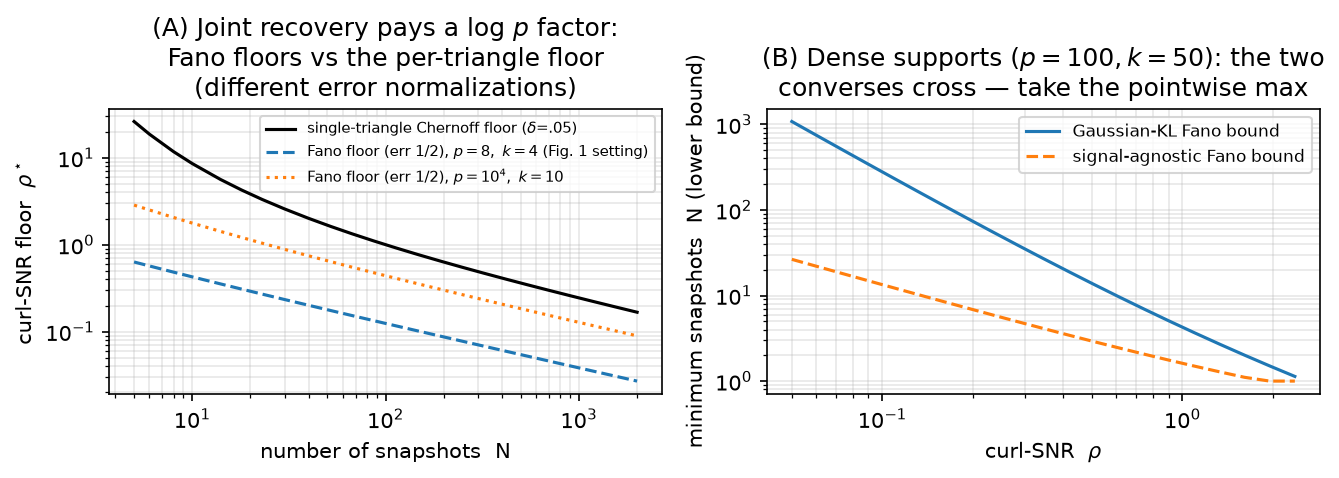
\includegraphics[width=\linewidth]{fano_bounds.png}
\caption{(A) Fano floors (Thm.~\ref{thm:fano-gauss}, inverted in $\rho$ at
error $1/2$) against the single-triangle Chernoff floor of the main paper.
(B) Dense-support regime: the Gaussian-KL and signal-agnostic bounds cross.
Script: \texttt{experiments/run\_fano.py}.}
\label{fig:fano}
\end{figure}

\section{Partial edge observation}\label{sec:partial}

Suppose only a subset $\mathcal E_{\mathrm{obs}}\subseteq\mathcal E$ of edges
is observed --- each edge independently with probability $q$ (Bernoulli
sampling). Write $\bm f_t^{\mathrm{obs}}$ for the observed sub-vector.

\begin{proposition}[Observability for curl statistics]\label{prop:obs}
The curl statistic $c_\tau=\B_2[:,\tau]^{\!\top}\bm f$ of candidate $\tau$ is
computable from $\bm f^{\mathrm{obs}}$ iff \emph{all three} edges of $\tau$
are observed. Under Bernoulli($q$) sampling each triangle is observable with
probability $q^3$, independently across edge-disjoint candidates.
\end{proposition}

An unobservable \emph{active} triangle is an automatic miss; an unobservable
\emph{inactive} one is an automatic correct rejection (the detector defaults
to ``inactive''). Combining with the exact per-triangle marginal laws (main
paper, Thm.~2) gives a closed form on edge-disjoint geometries:

\begin{corollary}[Exact recovery under edge sampling]\label{cor:qcubed}
With edge-disjoint candidates, the centered whitened detector at budget $N$
achieves
\begin{equation}\label{eq:qform}
\Pr[\hat\Scal=\Scal]
=\bigl[q^3\,(1-P_{\mathrm{miss}})\bigr]^{k}\;
\bigl[1-q^3P_{\mathrm{fa}}\bigr]^{p-k},
\end{equation}
where $P_{\mathrm{miss}},P_{\mathrm{fa}}$ are the $\chi^2_{N-1}$ error
probabilities of the fully observed test.
\end{corollary}
\begin{proof}
Independence of survival (Prop.~\ref{prop:obs}) and of the whitened scores
($\bm G=3\bm I$). An active triangle is recovered iff it survives
(prob.~$q^3$) \emph{and} is detected ($1-P_{\mathrm{miss}}$); an inactive one
is mislabeled iff it survives \emph{and} false-alarms ($q^3P_{\mathrm{fa}}$).
\end{proof}

The $q^{3k}$ factor is brutal: partial sampling multiplies the fully observed
recovery probability by $q^{3k}=q^{54}$ at $k=18$ active triangles --- a
factor $\approx 0.06$ at $q=0.95$ and $\approx 0.003$ at $q=0.9$ --- and the
Monte-Carlo cliff in Fig.~\ref{fig:partial}B follows the closed form within
sampling error. The restricted curve (recovery on the observable candidates
only) stays at~$\approx 1$ for all $q$: the bottleneck is purely coverage,
not detection.

\begin{remark}[Scope]\label{rem:partial-scope}
Proposition~\ref{prop:obs} is an \emph{operational} statement about detectors
built on curl statistics --- the class this paper analyzes. A triangle with
two observed edges still injects signal into those edges' flows, but that
signal is entangled with the unknown gradient nuisance once the exact curl
cancellation is unavailable; whether (and at what cost) it can be exploited,
e.g.\ by marginalizing the gradient over the observed sub-graph, is an open
question we do not claim to settle. Low-rank flow completion under sampling
(cf.\ graph sampling theory \cite{chen2015sampling}) is the natural attack.
\end{remark}

\begin{figure}[t]
\centering
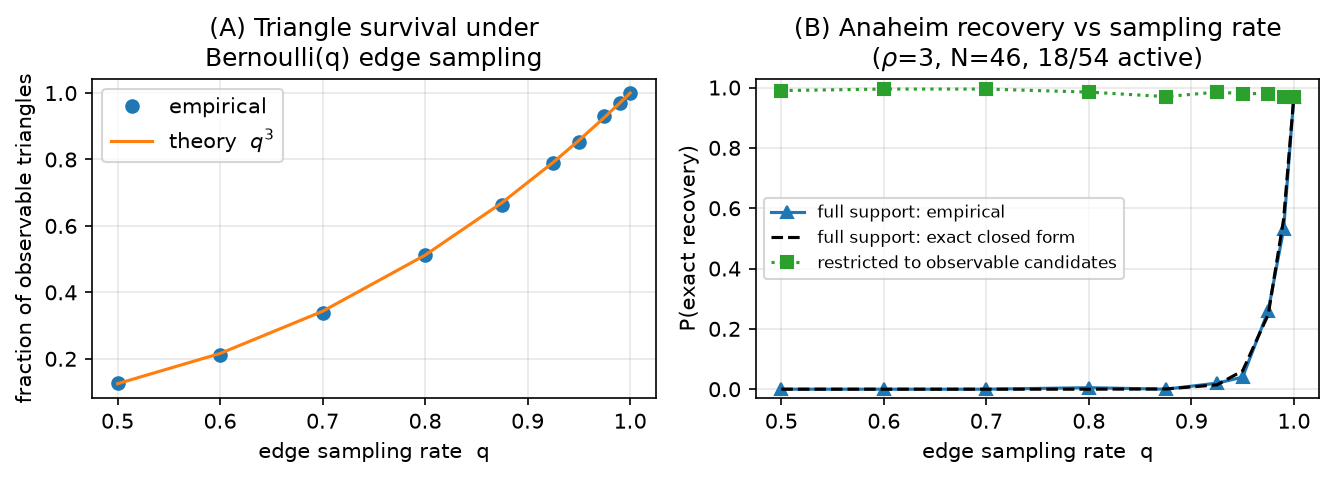
\includegraphics[width=\linewidth]{partial_sampling.png}
\caption{Partial edge observation on Anaheim (real geometry and equilibrium
flow background, $\rho=3$, $N=46$, $18/54$ active). (A) Triangle survival
follows $q^3$. (B) Full-support recovery collapses along the exact closed form
\eqref{eq:qform}; recovery restricted to observable candidates stays
$\approx 1$. Script: \texttt{experiments/run\_partial\_sampling.py}.}
\label{fig:partial}
\end{figure}

\section{Plug-in variance estimation and the adaptive detector}\label{sec:plugin}

The paper's detectors take $(\sigma_c,\sigma_n)$ as known. We now estimate
both from the same data. Let $u_\tau=\mathrm{score}_\tau/(\bm G^{-1})_{\tau\tau}$
denote the normalized whitened scores, so that for inactive $\tau$,
$N u_\tau/\sigma_n^2\sim\chi^2_{d}$ ($d=N$ or $N-1$ if centered), while active
scores are stochastically larger.

\paragraph{Estimators.}
\begin{align}
\hat\sigma_n^2 &= \frac{N\,\mathrm{med}_\tau(u_\tau)}{\mathrm{med}(\chi^2_d)},
\qquad\text{(median, robust to $<\!50\%$ contamination)}\label{eq:sn-hat}\\
\hat\sigma_c^2 &= \Bigl(\tfrac{1}{|\hat{\mathcal A}|}\textstyle\sum_{\tau\in\hat{\mathcal A}}
\bigl[\mathrm{score}_\tau-\hat v_{0,\tau}\bigr]\Bigr)_+,
\qquad\hat{\mathcal A}=\text{Bonferroni screen at level }\alpha,\label{eq:sc-hat}
\end{align}
followed by one refinement pass: after a first detection, $\sigma_n$ is
re-fit by the mean of the \emph{detected} off-support scores and $\sigma_c$ by
the on-support excess, and the detector is re-run once. Because the refit set
is selected by the same data, the refit is conditionally biased (missed
active triangles inflate $\hat\sigma_n$ --- measured $\approx +5\%$ at $N=10$
on the strip benchmark, vanishing for $N\ge 20$); its accuracy is established
empirically (Fig.~\ref{fig:plugin}A), not by an unbiasedness argument, and
Prop.~\ref{prop:plugin} applies conditionally on the deterministic error
bound $\epsilon$.

\begin{lemma}[Median consistency envelope]\label{lem:median}
Assume the candidates are pairwise edge-disjoint, so that the inactive
normalized scores are i.i.d.\ $\sigma_n^2\chi^2_d/N$ (the DKW step below
requires independence; for correlated scores the envelope is validated only
empirically). Let a fraction $\pi<1/2$ of the $p$ candidates be active and let
$\epsilon_p=\sqrt{\log(2/\delta)/(2(1-\pi)p)}$ satisfy $\pi+\epsilon_p<1/2$.
Then with probability at least $1-\delta$,
\[
q_{d}\!\left(\tfrac{1/2-\pi-\epsilon_p}{1-\pi}\right)
\;\le\; \frac{N\,\mathrm{med}_\tau(u_\tau)}{\sigma_n^2}
\;\le\; q_{d}\!\left(\tfrac{1/2}{1-\pi}+\tfrac{\epsilon_p}{1-\pi}\right),
\]
where $q_d(\cdot)$ is the $\chi^2_d$ quantile function. Consequently
$\hat\sigma_n^2/\sigma_n^2\in[q_d(\frac{1/2-\pi-\epsilon_p}{1-\pi}),
q_d(\frac{1/2+\epsilon_p}{1-\pi})]/q_d(1/2)$ --- an explicit, numerically
computable envelope that shrinks to $\{1\}$ as $p,d\to\infty$ whenever
$\pi<1/2$.
\end{lemma}
\begin{proof}
Active scores stochastically dominate inactive ones, so the sample median of
all $p$ scores is sandwiched between order statistics of the $(1-\pi)p$
inactive scores: at least a $(1/2-\pi)/(1-\pi)$-fraction and at most a
$(1/2)/(1-\pi)$-fraction of the inactive sample lies below it. The
Dvoretzky--Kiefer--Wolfowitz inequality applied to the inactive empirical CDF
converts these fractions into population $\chi^2_d$ quantiles up to
$\epsilon_p$, with probability $1-\delta$.
\end{proof}

\begin{proposition}[Plug-in perturbation]\label{prop:plugin}
Let the plug-in variances satisfy $\hat v_{i,\tau}=(1+e_{i,\tau})v_{i,\tau}$
with $|e_{i,\tau}|\le\epsilon<1/2$. Then each per-triangle error probability
of the adaptive detector exceeds its known-parameter counterpart by at most
$L_d\,\epsilon$, where $L_d<\infty$ is a Lipschitz constant of the
$\chi^2_d$ CDFs at the optimal threshold, and the exact-recovery probability
drops by at most $p\,L_d\,\epsilon$ (union bound).
\end{proposition}
\begin{proof}[Proof sketch]
The Bayes threshold $\gamma(v_0,v_1)$ of the two-variance test is a smooth
function of $(v_0,v_1)$ (main paper, Prop.~1), so
$|\hat\gamma-\gamma|\lesssim\epsilon\gamma$; the error probabilities are
integrals of bounded $\chi^2_d$ densities over the threshold shift.
\end{proof}

Empirically (Fig.~\ref{fig:plugin}) both estimates contract at the
$1/\sqrt N$ rate and the fully adaptive detector's recovery curve is
indistinguishable from the known-parameter detector for $N\gtrsim 30$ on the
confusable strip benchmark; the residual gap at $N\le 20$ (at most $0.06$
after refinement) is the price of estimating a variance from nine
medians.

\begin{figure}[t]
\centering
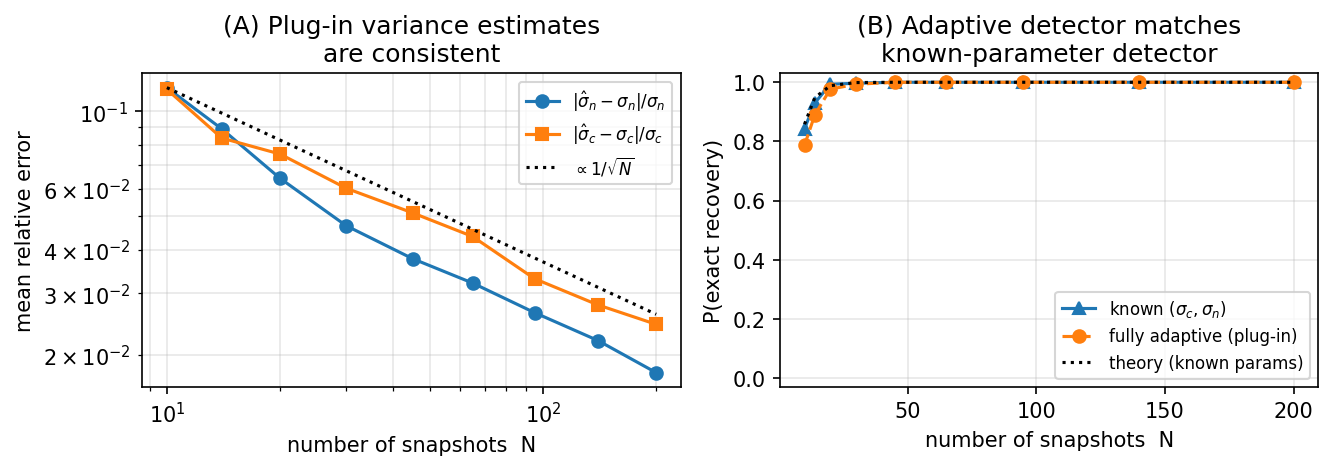
\includegraphics[width=\linewidth]{plugin.png}
\caption{Plug-in estimation on the strip benchmark of the main paper's
Fig.~2 ($\rho=8$, $4/9$ active). (A) Consistency of
\eqref{eq:sn-hat}--\eqref{eq:sc-hat} (after refinement). (B) The fully
adaptive detector matches the known-parameter detector.
Script: \texttt{experiments/run\_plugin.py}.}
\label{fig:plugin}
\end{figure}

\section{First- vs.\ second-order identifiability: proofs}\label{sec:dichotomy}

This section proves the main paper's Lemma~2 (lifted spark) and
Theorem~3 (first- vs.\ second-order dichotomy), and records the exhaustive
numerical verifications.
Here the candidate set is arbitrary (edge-sharing allowed, $\B_2$ possibly
rank-deficient); $\rho_2=\sigma_c^2/\sigma_n^2$ denotes the second-order SNR
(the per-triangle curl-SNR of the main text is $\rho=3\rho_2$).

\subsection{The lifted spark lemma}

\begin{lemma}[Lifted spark]\label{lem:spark-supp}
Let $\Tcal$ be any set of distinct $3$-cliques of a simple graph, with
signatures $\bm b_\tau\in\{0,\pm1\}^{|\mathcal E|}$ (columns of $\B_2$). The
matrices $\{\bm b_\tau\bm b_\tau^{\!\top}\}_{\tau\in\Tcal}$ are linearly
independent.
\end{lemma}
\begin{proof}
Fix $\tau=(i,j,k)$ and its edge pair $e=(i,j)$, $e'=(j,k)$. A pair of distinct
edges determines at most one triangle containing both (two edges sharing a
vertex fix the third vertex; disjoint edges lie in no common triangle). Hence
in $\bm A(\bm w)=\sum_{\sigma}w_\sigma\bm b_\sigma\bm b_\sigma^{\!\top}$, the
$(e,e')$ entry equals $w_\tau\,\bm b_\tau(e)\bm b_\tau(e')=\pm w_\tau$: no
other candidate contributes. $\bm A(\bm w)=\bm 0$ therefore forces
$w_\tau=0$ for every $\tau$.
\end{proof}

\begin{corollary}[Second-order identifiability]\label{cor:inject}
Under the main paper's model~(2), the map
$\Scal\mapsto\mathrm{Cov}(\bm f)=\sigma_g^2\B_1^{\!\top}\B_1
+\sigma_c^2\sum_{\tau\in\Scal}\bm b_\tau\bm b_\tau^{\!\top}
+\Sigma_{\rm harm}+\sigma_n^2\bm I$ is injective in $\Scal$; equivalently, in
the curl coordinate $\bm z=\bm Q^{\!\top}\bm f$ ($\bm Q$ an orthonormal basis
of $\mathrm{im}\,\B_2$, $r=\rank\B_2$),
\begin{equation}\label{eq:sigz}
\bm\Sigma_z(\Scal)=\sigma_n^2\bm I_r
+\sigma_c^2\!\!\sum_{\tau\in\Scal}\bm u_\tau\bm u_\tau^{\!\top},
\qquad \bm u_\tau=\bm Q^{\!\top}\bm b_\tau,
\end{equation}
determines $\Scal$ uniquely. (The gradient and harmonic covariance terms are
annihilated by $\bm Q^{\!\top}$; since $\bm b_\tau\in\mathrm{im}\,\B_2$, the
compression to curl coordinates loses nothing:
$\bm u_\sigma^{\!\top}\bm u_\tau=\bm b_\sigma^{\!\top}\bm b_\tau=G_{\sigma\tau}$.)
\end{corollary}

\subsection{First-order impossibility}

\begin{proposition}[Deterministic indistinguishability]
If $\mathrm{im}\,\B_{2,\Scal}=\mathrm{im}\,\B_{2,\Scal'}$ and the triangle
signals are unknown deterministic nuisance parameters, the families of flow
distributions $\{\mathcal N(\B_{2,\Scal}\bm y+\bm m,\ \sigma_n^2\bm I):\bm y\}$
and $\{\mathcal N(\B_{2,\Scal'}\bm y'+\bm m,\ \sigma_n^2\bm I):\bm y'\}$
coincide for every nuisance mean $\bm m$; consequently no test distinguishes
$\Scal$ from $\Scal'$ at any SNR and any $N$.
\end{proposition}
\begin{proof}
Equal column spaces: for every $\bm y$ there is $\bm y'$ with
$\B_{2,\Scal'}\bm y'=\B_{2,\Scal}\bm y$ and vice versa; apply per snapshot.
\end{proof}

Tetrahedral confusers realize the hypothesis: the four faces of a tetrahedron
satisfy $\bm b_{012}-\bm b_{013}+\bm b_{023}-\bm b_{123}=\bm 0$ (boundary of
the solid $3$-simplex), so any three faces span the same $3$-space as any
other three. On $K_n$ ($n\ge4$) there are $\binom n4$ tetrahedra.

\subsection{The price: exact separation and Chernoff exponent}

\begin{lemma}[Universal swap separation]\label{lem:sep16}
Let $\Scal'=\Scal\setminus\{\tau_a\}\cup\{\tau_b\}$ with $\tau_a,\tau_b$
faces of a common tetrahedron. Then
$\bm\Sigma_z(\Scal)-\bm\Sigma_z(\Scal')
=\sigma_c^2(\bm u_a\bm u_a^{\!\top}-\bm u_b\bm u_b^{\!\top})$ and
\[
\|\bm u_a\bm u_a^{\!\top}-\bm u_b\bm u_b^{\!\top}\|_F^2
=\|\bm u_a\|^4+\|\bm u_b\|^4-2(\bm u_a^{\!\top}\bm u_b)^2
=9+9-2=16 ,
\]
independent of $n$, of $|\Scal|$, and of the hosting tetrahedron (any two
faces share exactly one edge, so $\bm u_a^{\!\top}\bm u_b=G_{ab}=\pm1$).
\end{lemma}

\begin{proposition}[Chernoff exponent of the minimal confuser]\label{prop:cg}
Let $C_G$ be the Chernoff information between
$\mathcal N(\bm 0,\bm\Sigma_z(\Scal))$ and
$\mathcal N(\bm 0,\bm\Sigma_z(\Scal'))$ for a tetrahedral swap. As
$\rho_2\to0$,
\[
C_G=\tfrac{1}{16}\,\rho_2^2\,
\|\bm u_a\bm u_a^{\!\top}-\bm u_b\bm u_b^{\!\top}\|_F^2\,(1+o(1))
=\rho_2^2\,(1+o(1)),
\]
and the optimal error of the binary test from $N$ snapshots satisfies
$P_{\rm err}\le e^{-N C_G}$, with matching exponent
($\liminf_N -\tfrac1N\log P_{\rm err}=C_G$). Hence
$N^\star(\delta)\sim\log(1/\delta)/\rho_2^2$.
\end{proposition}
\begin{proof}[Proof sketch]
Write $\bm E=\bm\Sigma_0^{-1/2}(\bm\Sigma_1-\bm\Sigma_0)\bm\Sigma_0^{-1/2}$.
The Chernoff exponent between equal-mean Gaussians is
$\max_s\frac12[\log\det((1-s)\bm W_0+s\bm W_1)-(1-s)\log\det\bm W_0
-s\log\det\bm W_1]$; a second-order expansion in $\bm E$ around $\bm E=\bm 0$
is maximized at $s=1/2$ (Bhattacharyya) with value
$\tfrac1{16}\operatorname{tr}\bm E^2+O(\|\bm E\|^3)$. Here
$\bm E=\rho_2(\bm u_a\bm u_a^{\!\top}-\bm u_b\bm u_b^{\!\top})+O(\rho_2^2)$
(the shared atoms of $\Scal\cap\Scal'$ perturb $\bm\Sigma_0^{-1/2}$ only at
$O(\rho_2)$, entering $C_G$ at $O(\rho_2^3)$), so
$\operatorname{tr}\bm E^2=\rho_2^2\cdot16\,(1+O(\rho_2))$ by
Lemma~\ref{lem:sep16}. The bound $P_{\rm err}\le e^{-NC_G}$ is the Chernoff
bound; exponent tightness is classical for i.i.d.\ observations.
\end{proof}

\begin{proposition}[Fano over the confuser family]
On $K_n$, consider the $M=4\binom n4$ hypotheses obtained by choosing a
tetrahedron and leaving one of its four faces out of an otherwise-active
tetrad. Any estimator with error $\le\epsilon$ over the uniform prior needs
\[
N\ \ge\ \frac{(1-\epsilon)\log\!\big(4\tbinom n4\big)-\log 2}
{\max_{\text{pairs}}\KL\big(\bm\Sigma_z\|\bm\Sigma_z'\big)}
\ \asymp\ \frac{\log n}{\rho_2^2},
\]
i.e.\ full support recovery over the confuser family pays a $\log n$ factor
on top of the pairwise budget.
\end{proposition}

\subsection{Numerical verification (released tests)}

\texttt{tests/test\_second\_order.py} certifies, deterministically or by
Monte-Carlo: (i) Lemma~\ref{lem:spark-supp} on $K_4$--$K_9$, strips, disjoint
unions, and random clique complexes; (ii) injectivity of
$\Scal\mapsto\bm\Sigma_z(\Scal)$ \emph{exhaustively} over all $2^4$ supports
of $K_4$; (iii) the deterministic replication of first-order confusers
(residual $<10^{-9}$); (iv) separation exactly $16$ for every tetrahedral
swap, and (exhaustively on $K_5$, all support sizes $k\le5$) minimality of
$16$ over \emph{all} equal-image pairs; (v)
$C_G/\rho_2^2\in[0.95,1.005]$ for $\rho_2\le10^{-2}$ and the Monte-Carlo
error of the optimal test within the $e^{-NC_G}$ envelope with empirical
exponent decreasing onto $C_G$; (vi) exact greedy covariance-atom recovery on
rank-deficient $K_5$ (the regime where first-order arguments forbid it).

\section{The cyclone study: construction details}\label{sec:cyclone}

This section records the methodological details of the main paper's
real-data recovery experiment (Fig.~3 there) beyond what fits in the page
budget.

\paragraph{From winds to edge flows.} ERA5 10\,m winds (ARCO-ERA5 public
archive, $0.703^\circ$ equiangular grid, 6-hourly), Western North Pacific
($0$--$45^\circ$N, $100$--$180^\circ$E), Aug--Sep 2020 (244 snapshots; the
season contains 13 IBTrACS storms, incl.\ Bavi, Maysak, Haishen). Mesh nodes
subsample every third grid point ($\approx2.1^\circ$); each grid cell splits
into two right triangles; edge flow $=$ trapezoidal line integral
$\tfrac12(\bm V_i+\bm V_j)\!\cdot\!(\Delta x,\Delta y)$ in the local
equirectangular metric ($\Delta x = R\cos(\bar\phi)\Delta\lambda$). The mesh
is simply connected, so $\#\text{triangles}=|\mathcal E|-|\mathcal V|+1
=\dim\ker\B_1$ and $\B_2$ has full column rank (verified: $1554/1554$) --- the
favorable-geometry regime of the dichotomy, with no equal-image confusers.
By Stokes' theorem the curl statistic of a triangle approximates its
circulation, i.e.\ area-integrated relative vorticity; a sign convention
(sorted-vertex traversal vs.\ geometric orientation) is tracked explicitly in
the code and is irrelevant to the energy detector.

\paragraph{Detection.} Per 4-day window (16 snapshots), the temporally
centered decorrelated scores $\hat{\bm y}=\bm G^{-1}\bm c$ are computed with
NO oracle parameters: centering removes any window-constant background
exactly, and thresholds/scales are plug-in (\S\ref{sec:plugin} machinery).
Windows are the device that maps the i.i.d.-snapshot theory onto moving
weather: a cyclone translates $\sim$$3$--$6^\circ$/day, so over 4 days it
crosses a few $2.1^\circ$ triangles --- the "support" is quasi-static at the
window scale, and the per-window scores are pooled across the season for
evaluation. This is an idealization and is labeled as such (README honesty
note 9).

\paragraph{Validation.} Internal: relative vorticity
$\zeta=\partial_x v-\partial_y u$ by centered differences on the FULL
$0.7^\circ$ grid (the detector only ever sees the $2.1^\circ$ mesh flows);
per-triangle truth $=$ window-mean $|\zeta|$ averaged over grid points inside
the triangle; ROC sweeps the detector score against truth binarized at
typhoon-scale $3\times10^{-5}\,\mathrm{s}^{-1}$. External: IBTrACS v04r01
best-track fixes ($\ge$ 34\,kt where wind is reported), a triangle labeled
positive if a fix falls within $1.5^\circ$ of its centroid during the window.
The external reference shares nothing with ERA5's assimilation of winds into
our statistic --- it is the community's independent record of where cyclones
actually were. A synthetic Rankine-vortex test (\texttt{tests/test\_geo.py})
verifies the whole bridge end-to-end: localization at the core, correct
cyclonic sign after orientation correction, and rank agreement with the
finite-difference vorticity.

\section{Reproducibility}\label{sec:repro}

All figures regenerate on CPU from fixed seeds via
\texttt{experiments/run\_all.py}; individually:
Fig.~\ref{fig:fano} $\leftarrow$ \texttt{run\_fano.py} (pure theory, seconds);
Fig.~\ref{fig:partial} $\leftarrow$ \texttt{run\_partial\_sampling.py}
($\approx$4\,min);
Fig.~\ref{fig:plugin} $\leftarrow$ \texttt{run\_plugin.py} ($\approx$3\,min);
the main paper's cyclone study $\leftarrow$ \texttt{run\_real\_cyclone.py}
($\approx$3\,min from the cached ERA5/IBTrACS files).
The test-suite (\texttt{pytest -q}, 34 tests) checks: the Fano bounds against
the empirical recovery boundary of the main paper's Fig.~1 (a converse must
lower bound it), the closed form \eqref{eq:qform} against Monte-Carlo, the
envelope of Lemma~\ref{lem:median}, the adaptive-vs-known recovery gap, every
claim of Section~\ref{sec:dichotomy} (spark, exhaustive $K_4$ injectivity,
separation $16$, $C_G/\rho_2^2\to1$, Chernoff envelope, rank-deficient
recovery), and the wind-to-edge-flow bridge (mesh full rank by Euler; a
synthetic Rankine vortex localizes at the correct triangles with the correct
sign and matches the finite-difference vorticity ranking).

\begin{thebibliography}{9}
\bibitem{vershynin2018high}
R.~Vershynin, \emph{High-Dimensional Probability}, Cambridge Univ.\ Press, 2018.
\bibitem{chen2015sampling}
S.~Chen, R.~Varma, A.~Sandryhaila, and J.~Kova\v{c}evi\'c,
``Discrete signal processing on graphs: Sampling theory,''
\emph{IEEE Trans.\ Signal Process.}, vol.~63, no.~24, pp.~6510--6523, 2015.
\end{thebibliography}

\end{document}
